\section{Detecting Flaky Tests}
\label{sec:detectFlakyTests}

The detection of flaky tests is a crucial aspect of software testing and development. This process not only protect resources by preventing wasted efforts on resolving misleading failures but also influences software release timelines by providing clearer insights into test outcomes. When test failures are accurately identified as flaky, developers can make more efficient release decisions and avoiding unnecessary delays. My motivation to work in this field falls in the significance of flaky test detection in enhancing software development processes and quality. My goal is to analyze existing detection techniques, assess their strengths and limitations, and use these insights to propose more detection techniques. 

Running tests many times is the traditional way to find flaky tests. Unfortunately, there is little industrial and academic guidelines regarding how many times to rerun each test in order to check if there are flaky or not. Prior studies consider many different numbers to run each test such as 10 \cite{bell2018deflaker}, 16 \cite{lam2019idflakies}, 100 \cite{lam2019root} or, 4,000 times \cite{lam2020Understanding}.
As there are various non-deterministic reasons behind flaky tests, it is hard to claim that developers will observe test flakiness within a fixed number of runs. 
Running tests could not be a major problem if developers can ensure that within e.g. 5 runs flaky tests can be detected.
Another problem related to rerun is that it could be hard to reproduce the flaky failure detected in the original environment using another environment (e.g. developers who locally debug flaky tests which failed on a server). This problem of reproducing flaky tests is due the lack of knowledge about the non-deterministic source that cause flaky failures whether it is due to Java version, network speed, etc. 


Alternatively, I am proposing \sysName, a Machine Learning (ML) approach to identify which tests in a test suite are flaky, \emph{without} rerunning them many times. \sysName learns from existing flaky tests in order to predict unseen tests if they are flaky or not. \sysName can be used to search for flaky tests in a large test suite, where developers identify that a portion of the test suite is or is not flaky, and use \sysName to help label the rest of the tests as flaky or not. Also, \sysName could help in terms \emph{prioritize} which tests should be run first by reporting which tests are most likely to be flaky. 


By proactively identifying flaky tests, I may also help developers understand why these tests are flaky.
Prior work has suggested different properties of tests that might make them more likely to be flaky, and \sysName can report which of these features are present in each test~\cite{eck2019understanding,ahmad2021empirical}.
In practice, if a feature has a strong correlation with flakiness, developers might choose to focus on this feature in their future test maintenance and development activities. 



\subsection{RERUN: Empirical Study}
\label{sec:flakeFlaggerStudy}
%
% This section is a summary of the study conducted in my paper ``FlakeFlagger: Predicting Flakiness Without Rerunning Tests" published in ICSE2021 \cite{alshammari2021flakeflagger}.

% I am motivated to conduct this study in order to answer these main research questions:

% \begin{itemize}
% \setlength{\itemindent}{3em}
% \item[\textbf{RQ1:}]
% How many flaky tests can be found by rerunning tests given different rerun budgets?
% \item[\textbf{RQ2:}] 
% How hard is it to reproduce a flaky test failure? 

% \end{itemize}

% \subsubsection{Study Design}
To gather data on flaky tests, 24 Java projects were selected and run, some of which had been previously studied for test flakiness using different revisions \cite{bell2018deflaker} \cite{lam2019idflakies}. The entire test suites of these projects were run 10,000 times, which differed from the previous work \cite{bell2018deflaker} \cite{lam2019idflakies}. Only a single revision of each project was considered, which was either the most recent revision at the time of writing or the same revision studied in \cite{bell2018deflaker} or \cite{lam2019idflakies}.

The rerun scripts were used to break down large experiments into smaller units called "jobs," which were executed on virtual machines. A single job was the execution of a Java test suite on a specific revision of a project using the Maven build system. For each job, the Maven build log and XML reports for each test run were saved. This approach aimed to create a level of isolation between test runs and simulate how an actual integration server would compile, test, and run a project's test suite.


The method I used to detect flaky tests through rerun is not the only approach available. There are other ways to increase the likelihood of detecting flaky tests. For instance, some flaky tests can be affected by the order in which they are run, and running them in different orders may uncover additional flaky tests \cite{lam2019idflakies}. However, this may also introduce a bias towards certain categories of flaky tests. Another way to detect more flaky tests is to run the experiment on different platforms and devices. However, my goal was to align the rerun experiment with standard development practices.


\subsection{FlakeFlagger: Flaky Test Classifier}
\label{sec:flakeFlaggerClassifier}

This section focuses on the construction process of the \sysName, beginning with the feature collection, followed by the classification process, and finally detailing how all of these elements have been designed as illustrated in Figure~\ref{over_all_graph}.


\begin{figure*}[t]
%\captionsetup{singlelinecheck = false, justification=justified}
  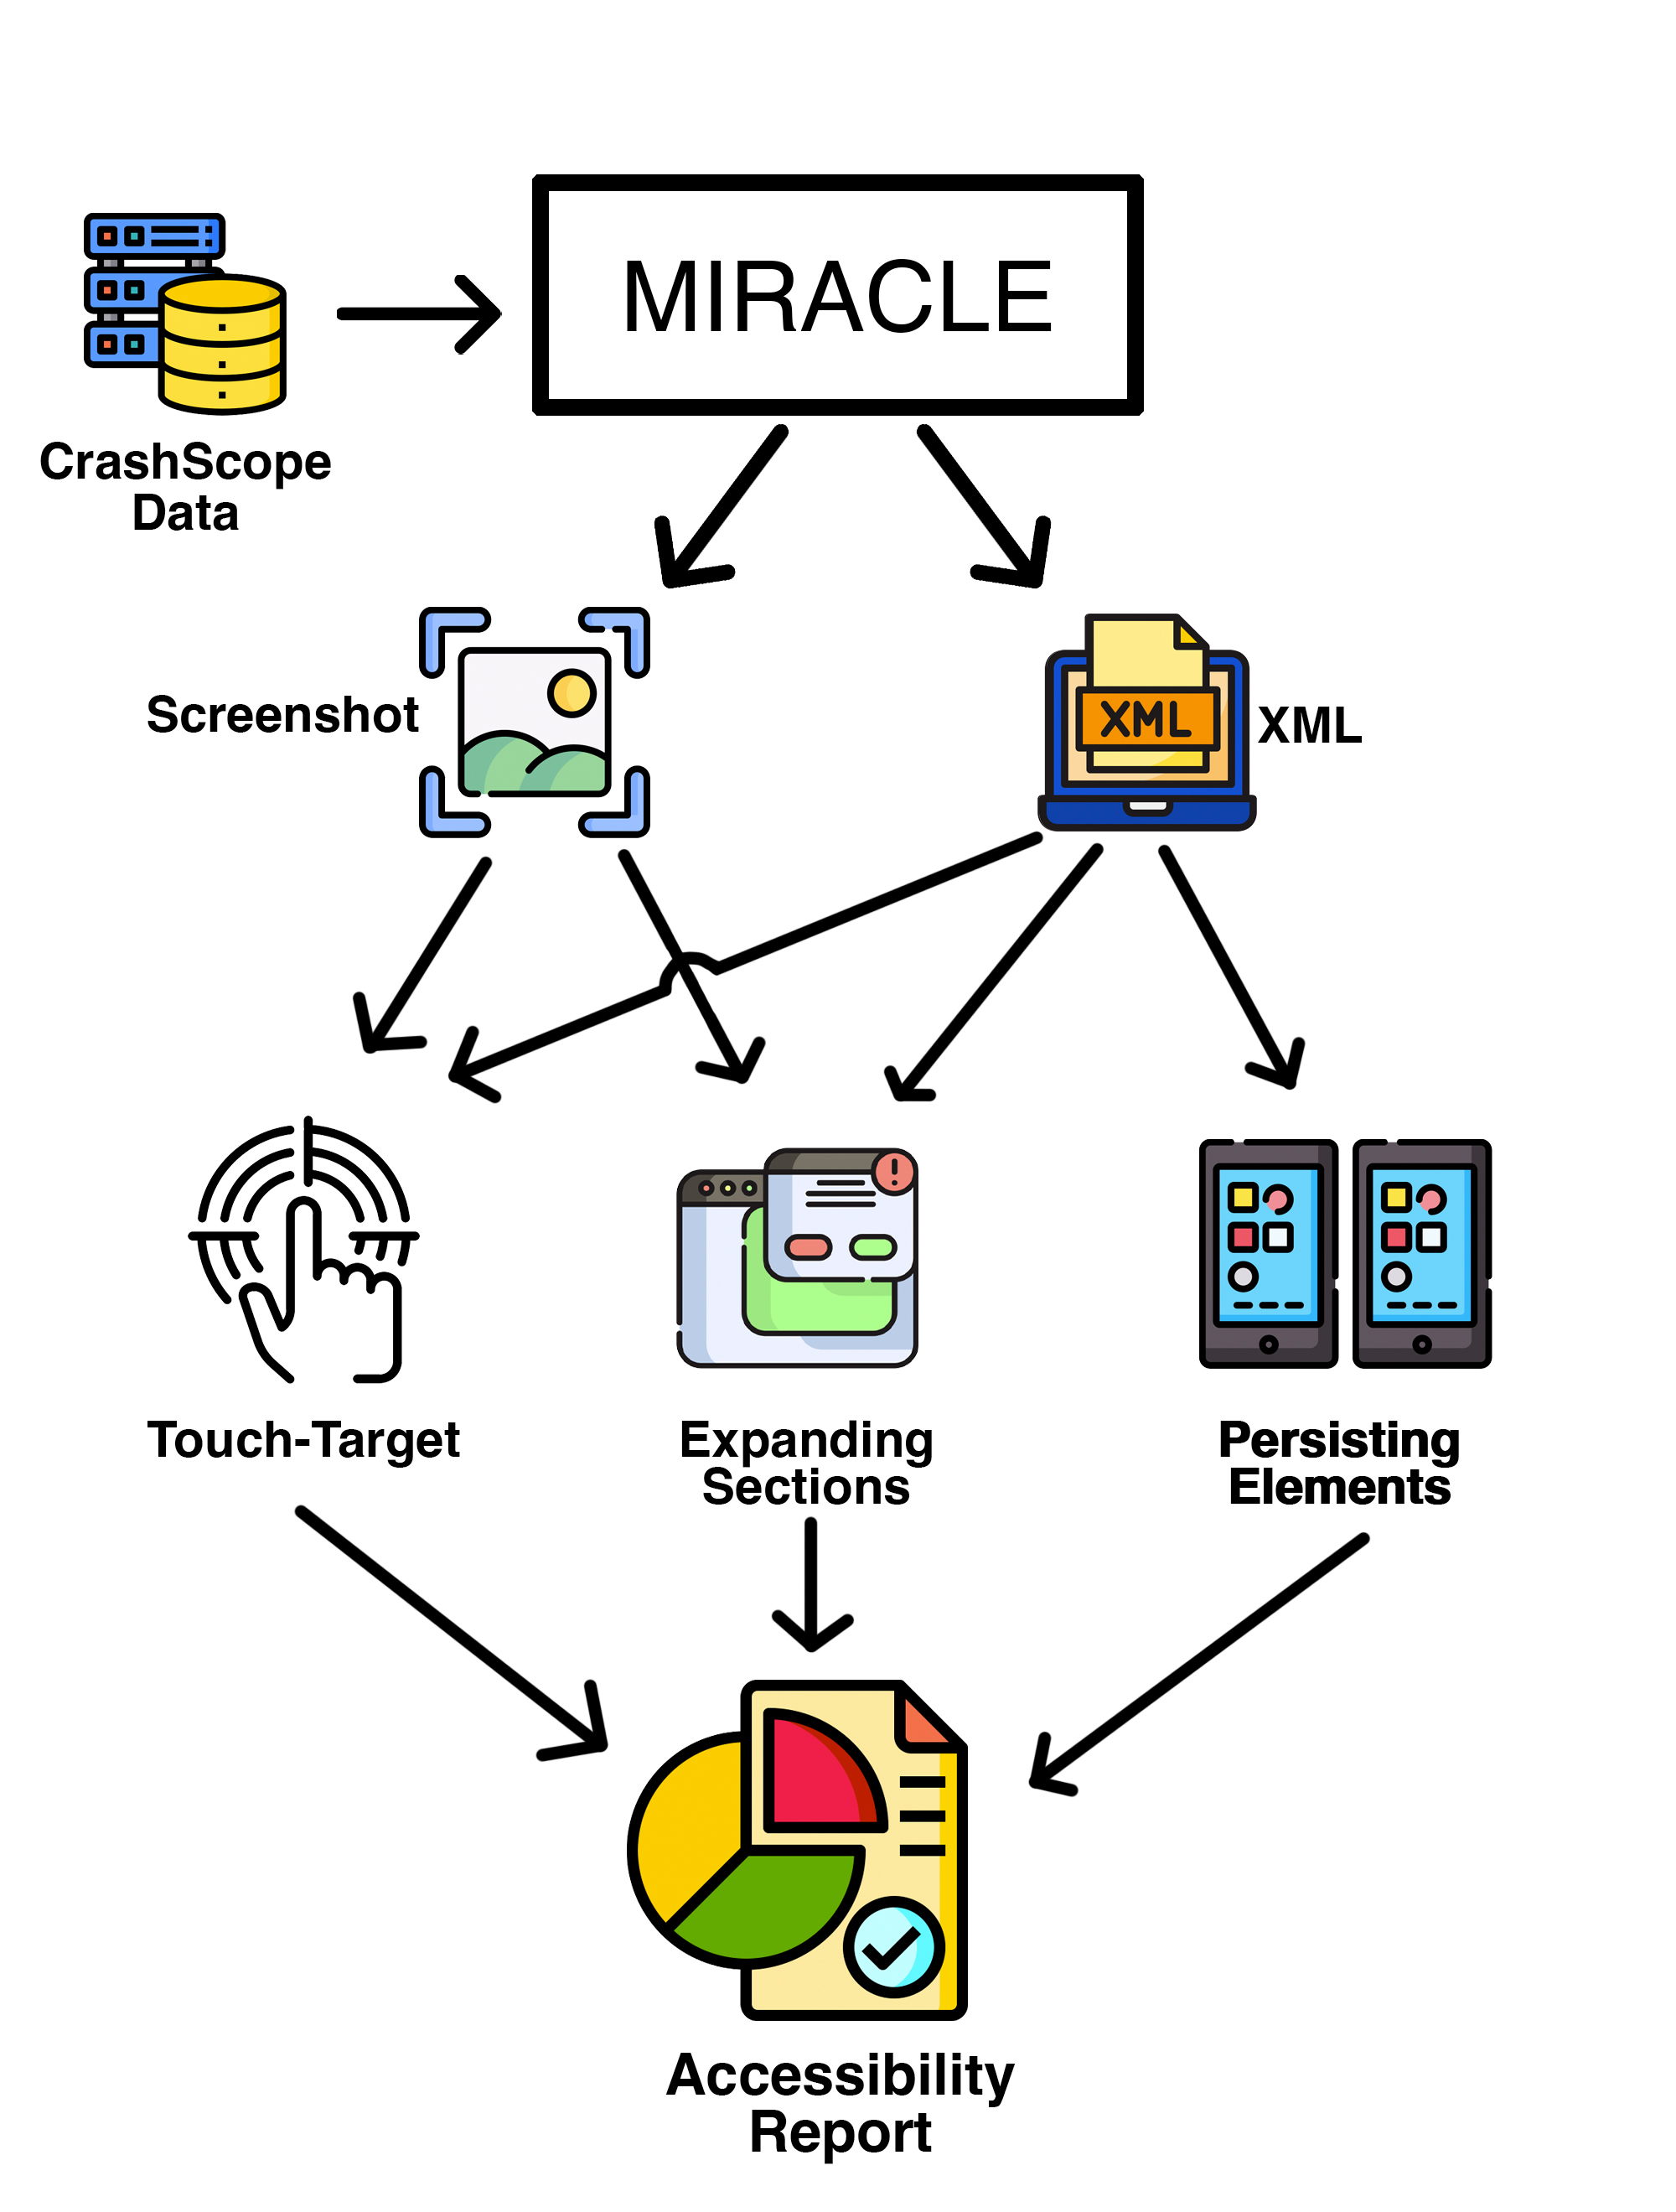
\includegraphics[width=0.9\textwidth]{Figures/overview.pdf}
  \centering
  \vspace{-5pt}
  \caption{Overview of \sysName's approach to predict likely flaky tests.}
  \vspace{-15pt}
  \label{over_all_graph}
\end{figure*}
\vspace{-5pt}

% This section is a summary of the \emph{approach} section in my paper ``FlakeFlagger: Predicting Flakiness Without Rerunning Tests" published in ICSE2021 \cite{alshammari2021flakeflagger}.



\subsubsection{Features Collections}
\label{sec:detector}
Machine learning classifiers such as \sysName require a set of feature in order to learn and predict. I started with the prior work \cite{luo2014empirical,eck2019understanding,bell2018deflaker} to study which features is highly linked to flakiness. I aim to collect verity of features because of the fact that some flaky tests in different projects often have different root causes for their flakiness\cite{luo2014empirical}. Similarly, some features that are predictive for one project may not be as predictive for others, due to the inherent non-determinism in flaky tests. 
I intentionally collect some dynamic features, in addition to static features (e.g. presence of textual tokens in the body of each test method). This is important because some causes not in the test method itself, but instead, in the production code that is executed by that test \cite{eck2019understanding}.
Ahmed et al. \cite{ahmad2021empirical} categorized 23 developer-reported factors which affect test flakiness. 
These features are described by practitioners at a high level, and include test case complexity, hard-coded values and test smells.
Eck et al. \cite{eck2019understanding} interviewed 21\Space{ professional} developers about flaky tests and tabulated the frequency of different kinds of flaky tests as well as developers' fixes for those flaky tests. 


Inspired by previous studies on test flakiness, I developed a list of sixteen features, 
some of are based on general studies on the causes of flaky tests \cite{luo2014empirical,ahmad2021empirical}, while others are defined as bad practices in writing unit tests.
Hence, I considered all of the features described in the prior works, and then selected only those for which I could write automated detectors.
This ends up with implementing detectors for each of the features shown in Table \ref{table:Feature_desc}. This list of features is not intended to be complete: there may yet be other features that can be easily collected and will be useful for predicting test flakiness.

While some of the features can be detected by inspecting the test method statically (specifically, the conditional logic smell and test line of code), the rest of the features require more than static analysis.
A hybrid static/dynamic framework \emph{detector} was developed to collect the statement coverage of each test, and then statically analyze the covered code in order to collect these behavioral features.
The \emph{detector} also collect a variety of other features related to the statement coverage of each test, such as how many recently changed lines of code are covered.
The \emph{detector} is implemented as an extension to the Maven build system.


\begin{table*}[t]
\scriptsize
%\renewcommand{\arraystretch}{1.3}
    \caption[FlakeFlagger List of Collected Features.]{Complete list of features captured for test flakiness prediction. The Covered Lines Churn feature is represented in multiple forms based on the $h$ values (number of the past commits). In the evaluation, I considered $h=5, 10, 25, 50, 75, 100, 500$ and $10,000$}
    \vspace{-5pt}
    \label{table:Feature_desc}
    \begin{tabularx}{\textwidth}{l | l X}
    \toprule
    & \bfseries Feature & \bfseries Description\\
    \midrule
\parbox[t]{2mm}{\multirow{8}{*}{\rotatebox[origin=c]{90}{Test Smells}}}	&
	Indirect Testing  	&	 True if the test interacts with the object under test via an intermediary \cite{van2001refactoring}  \\
	&	Eager Testing 	&	 True if the test exercises more than one method of the tested object \cite{van2001refactoring} \\
	&	Test Run War  	&	 True if the test allocates a file or resource which might be used by other tests \cite{van2001refactoring} \\
	&	Conditional Logic 	&	 True if the test has a conditional if-statement within the test method body \cite{meszaros2007xunit} \\
	&	Fire and Forget  	&	 True if the test launches background threads or tasks. \cite{garousi2018smells} \\
	&	Mystery Guest 	&	 True if the test accesses external resources  \cite{van2001refactoring} \\
	&	Assertion Roulette  	&	 True if the test has multiple assertions \cite{van2001refactoring} \\
	&	Resources Optimism  	&	 True if the test accesses external resources without checking their availability \cite{van2001refactoring}\\ \hline
\parbox[t]{2mm}{\multirow{8}{*}{\rotatebox[origin=c]{90}{Numeric Features}}}	&	Test Lines of Code   	&	 Number of lines of code in the test method body \\
	&	Number  of Assertions  	&	 Number of assertions checked by the test \\
	&	Execution Time   	&	 Running time for the test execution \\
	&	Source Covered Lines  	&	 Number of lines covered by each test, counting only production code \\
	&	Covered Lines  	&	 Total number of lines of code covered by the test  \\
	&	Source Covered Classes  	&	 Total number of production classes covered by each test \\
	&	External Libraries  	&	 Number of external libraries used by the test \\
	&	Covered Lines Churn 	&	 $h$-index capturing churn of covered lines in past 5, 10, 25, 50, 75, 100, 500, and 10,000 commits. Each value $h$ indicates that at least $h$ lines were modified at least $h$ times in that period.\\
\bottomrule
    \end{tabularx}
    % \vspace{-14pt}
\end{table*}

% \begin{table*}[t]
% \begin{tabular}{l l l}
% & Indirect Test Smell & Testing blah\\
% \end{tabular}
% \end{table*}

\subsubsection{Classification Process}

FlakeFlagger takes a list of tests, where each of them is represented as a vector $\{x_1, x_2, x_3,\dots, x_n\}$  where each \emph{x} represents a feature value and \emph{n} correspond the total number of features. I applied data inspection and cleaning process to make that dataset more clear for the classification. Missing data can exist to the dataset due to the fact that some features collected by the detector can be incomplete e.g. due to crashes in the middle of the test execution. Some tests are not written in Java, and hence the feature detectors may not be applicable to them, and due to inheritance, some tests may not have source code in the project under test.

As in any classification problem, considering multiple supervised learning algorithms could be better. In \sysName, it is designed to use a set of models including Random Forest (\emph{RF}) and Decision Tree (\emph{DT}. I follow a feature selection process using \emph{information gain}, which computes the amount of information that a feature can provide for a classification \cite{lei2012feature}. Imbalanced datasets (where there is not an equal number of instances in each class --- flaky and non-flaky tests in my case) usually have very low information gain values. 


\subsubsection{Experimental Design}
\label{sec:Prediction_Design}
To evaluate \sysName, I used the same dataset described in Section \ref{sec:flakeFlaggerStudy}. I ran the detector described in Section \ref{sec:detector}, to collect the set of features shown in Table \ref{table:Feature_desc}. \sysName, similar to any machine learning classifiers, relies on two data sets: one to build the model (training) and another for testing. Because this is not already designed and I have only one dataset, I applied $k$-fold cross validation \cite{kohavi1995study} to evaluate the model. Following this practice, I split the data into $k$ parts, leave one part for testing and $k-1$ to train the classifier.
I then repeat this process with another $k-1$ parts, each time leaving one part for testing.
However, $k$-fold cross validation is most applicable to data that is evenly balanced, where the proportions of each class (flaky and not flaky) are similar. In fact, most tests are not flaky, which means imbalance data. To overcome this, I applied a sample technique SMOTE \cite{SMOTE} only on training dataset, to ensure a valid and fair result.



In my prediction evaluation, I label each prediction result as a True Positive (TP), False Negative (FN), False Positive (FP), or True Negative (TN) as follows:
TP - predicted flaky, known to be flaky; FP - predicted flaky, not known to be flaky; FN - predicted not flaky, known to be flaky; TN - predicted not flaky, not known to be flaky.
I also evaluate the models using F1-score, which is computed using the standard formula based on Recall and Precision. %, to evaluate how our approach works to detect flaky tests as $TP$s.
%  \abdul{I added the following sentences ... } JB: Looks good!
Lastly, I calculate the Area Under the Curve (AUC), a measure of how effective a model is at distinguishing classes.
% (in my case, flaky and not flaky).

In the evaluation, false positives represent the number of tests that might be considered as flaky by developers, resulting in excess effort spent re-running them to determine if they are flaky or not. I focus primarily on total positives, because I have confidence that the collected flaky tests are indeed flaky, but I cannot be confident in my classification of a test as not flaky. 
In other words, the oracle is a result of detecting flaky tests after \numruns~runs for each test, but this does not guarantee that the ``not flaky'' tests are really not flaky: they may just not have been observed to be flaky. 
This approach also allows us to confirm $FN$s are truly flaky tests because they fail at least once during rerun tests.
However, because of the inherent non-determinism in flaky tests, I cannot construct a reliable oracle to evaluate $TN$s and $FP$s, but report them as-is.








\subsection{Evaluation}
I evaluate my findings in detecting flaky tests by answering the following  main research questions:


\begin{description}
  \item[\textbf{RQ 4.3.1:}] How many flaky tests can be found by rerunning tests given different rerun budgets?
  \item[\textbf{RQ 4.3.2:}] How hard is it to reproduce a flaky test failure?

  \item[\textbf{RQ 4.3.3:}] How effective is \sysName at predicting flaky tests?
  \item[\textbf{RQ 4.3.4:}] How helpful is each feature in distinguishing between flaky and non flaky tests?
  
 \end{description}



By running each test 10,000 times, 811 flaky tests were detected: about \flakytestsrate\% of the total number of tests were flaky. The number of flaky tests in 24 projects are not equally distributed. For example, \projectsout~projects with less than 10 flaky tests, \projectsoneflaky~of which have only one, and one with none. On the other hand, there are \projectshundredsflaky~projects which have more than 100 flaky tests. \emph{Spring-boot} has \springbootFlaky~flaky tests, \highestflakyrate\% of the total observed flaky tests. Table \ref{table:rerun_result} summarizes these results. 

\subsubsection{How many flaky tests can be found by rerunning tests given different rerun budgets?} 
\label{FlakeFlaggerRQ1}

I calculated the probability that each flaky test would have been detected with fewer reruns. It is important to consider that it is not possible to state the probability due to the fact that there could be uncontrolled unaware conditions that cause the failure. As a result, only roughly a quarter of all of the flaky tests that I found in 10,000 runs would have been found with 10 reruns, roughly half with 100 reruns and roughly two thirds with 1,000 reruns.

Table \ref{table:rerun_result} categorizing each flaky test as failing either between 0 and 10 times, between 10 and 100 times, between 100 and 1,000 times, and finally over 1,000 times (out of the 10,000 runs).
These sets are represented by colors as shown in Table \ref{table:rerun_result}. The \emph{red} bar, which refers to tests that flake less than or equal 10 times, takes the majority in \redbarsratio~projects. 
In general, I found more than \NumFailingRunsTen\% of total flaky tests fail in less than or equal 10 times, \NumFailingRunsHundred\% of flaky tests fail more than 10 and less than or equal 100 out of 10,000.
This suggests that flaky tests datasets with limited runs still not ensure to detect \emph{most} flaky tests.
Furthermore, I acknowledge that even after 10,000 re-runs, it is still possible that all flaky tests in this dataset have been detected. 

\subsubsection{How hard is it to reproduce a flaky test failure?}
\label{FlakeFlaggerRQ2}

In the previous \textbf{RQ}, the rerun experiment aims to study the difficulty of identifying flaky tests by re-running them on the same platform. However, this does not capture the difficulty when a developer rerun the tests on different environment e.g. local machine. to meet this, I compared the set of flaky tests identified from the 10,000 reruns with those detected by prior researchers on the same versions of the same projects, but in different environments.
The columns \emph{DeFlaker} and \emph{iDFlakies} in Table \ref{table:rerun_result} show the total number of flaky tests that that paper reported on that version of that project, along with the number of those tests that were also found to be flaky based on the reruns.
A blank entry indicates that the revision of that project that I executed did not have any flaky tests reported by the prior work.
The DeFlaker dataset contains flaky tests from many revisions of each project, but I only studied a single revision of each project, and hence, it is possible that DeFlaker had not identified any flaky tests in that revision.
The iDFlakies dataset consists of both order dependent tests (which are detected by shuffling execution orders), and non-order dependent tests (which are flaky regardless of execution order).
Since I purposefully did not shuffle the execution order of the tests (as described above), I include only the non-order dependent tests from iDFlakies for comparison. 

Comparing to DeFlaker, I found \deflakerCommonFlaky~flaky tests out of the \deflakerRerunFlaky~tests identified as flaky by DeFlaker.
Unfortunately, the DeFlaker authors did not retain the build logs from their test runs, so I are unable to diagnose why those tests appeared as flaky to DeFlaker but not to my reruns.
Comparing to iDFlakies, I found \idflakiesCommonFlaky~flaky tests out of the \idflakiesRerunFlaky~non-order dependent tests that I reran.
In the case of iDFlakies, the authors \emph{did} retain the build logs that show how these tests failed, and I confirmed by hand that the tests that I missed in my rerun experiment truly were flaky, and could have been detected as flaky if I had rerun them more.
These results are indicative of the true non-determinism of flaky tests and the difficulties that developers face reproducing them: even with 10,000 reruns, I could not detect all flaky tests.





%  the new table 3 

\begin{table*}[t]
 \setlength{\tabcolsep}{1.6pt}

\caption[FlakeFlagger Prediction Result.]{Prediction performance for \sysName, the \vocabName, and the hybrid combination of both.
\textnormal{The hybrid approach builds a model with both \sysName's and the \vocabName's features. I show the number of True Positives, False Negatives, False Positives and True Negatives, Precision, Recall, and F1 scores per-project.
The AUC value is calculated after each fold where the reported value is the overall averages of AUC values after all folds. Projects with zero F1 values have very low numbers of flaky tests (less than 3 per project), and illustrate known limitations of \sysName. } }
%\caption{Prediction performance for \sysName, MSR and the combination between two approaches. 
% \textnormal{For \sysName, showing True Positives, False Negatives, False Positives, True Negatives, Precision, Recall and F1-score. For comparison approaches (FLAST \cite{flast} at $\sigma=0.5$ and $\sigma=0.95$ and random guessing with 50\% probability of flakiness or weighted by the distribution of flaky tests in the project), we show only Precision, Recall and F1-score. Highest F1-score in each row is shown in bold. Since each project uses a different model, we do \emph{not} include a ``total'' row.}
%}
\label{table:Full_result}
\vspace{-5pt}
\resizebox{\textwidth}{!}{
% \scriptsize
\begin{tabular}{l rr| rrrrrrr | rrrrrrr | rrrrrrr}

\toprule
% & \multicolumn{4}{c|}{} & \multicolumn{4}{c|}{\textbf{MSR tool *}} & \multicolumn{4}{c}{\textbf{Both}}\\
% \cmidrule(lr){2-5} \cmidrule(lr){6-10}
& & \textbf{Flaky by} & \multicolumn{7}{c|}{\textbf{\sysName}} & \multicolumn{7}{c|}{\textbf{Vocabulary-Based Approach \cite{pintovocabulary}}} & \multicolumn{7}{c}{\textbf{Combined Approach}}  \\
\cmidrule(lr){4-10} \cmidrule(lr){11-17}  \cmidrule(lr){18-24}
% \cmidrule(lr){2-14} \cmidrule(lr){10-13} \cmidrule(lr){14-17} \cmidrule(lr){18-21} 


\textbf{Project} & \textbf{Tests} & \textbf{Reruns} &\textbf{TP} & \textbf{FN} & \textbf{FP} & \textbf{TN} & \textbf{Pr} & \textbf{R} & \textbf{F} & \textbf{TP} & \textbf{FN} & \textbf{FP} & \textbf{TN} & \textbf{Pr} & \textbf{R} & \textbf{F} &  \textbf{TP} & \textbf{FN} & \textbf{FP} & \textbf{TN} & \textbf{Pr} & \textbf{R} & \textbf{F}\\
\midrule
spring-boot& 2,108 & 160 & 139 & 21 & 15 & 1,933 & 90\% & 87\% & 89\% & 134 & 26 & 703 & 1,245 & 16\% & 84\% & 27\% & 143 & 17 & 18 & 1,930 & 89\% & 89\% & 89\% \\
\rowHighlight hbase &431 & 145& 129 & 16 & 32 & 254 & 80\% & 89\% & 84\% & 89 & 56 & 152 & 134 & 37\% & 61\% & 46\% & 130 & 15 & 33 & 253 & 80\% & 90\% & 84\% \\
alluxio & 187 & 116& 116 & 0 & 0 & 71 & 100\% & 100\% & 100\% & 108 & 8 & 11 & 60 & 91\% & 93\% & 92\% & 116 & 0 & 0 & 71 & 100\% & 100\% & 100\% \\
\rowHighlight okhttp & 810 &100 & 52 & 48 & 159 & 551 & 25\% & 52\% & 33\% & 79 & 21 & 444 & 266 & 15\% & 79\% & 25\% & 46 & 54 & 104 & 606 & 31\% & 46\% & 37\% \\
ambari & 324 & 52& 47 & 5 & 3 & 269 & 94\% & 90\% & 92\% & 36 & 16 & 121 & 151 & 23\% & 69\% & 34\% & 47 & 5 & 3 & 269 & 94\% & 90\% & 92\% \\
\rowHighlight hector & 142 & 33 & 30 & 3 & 8 & 101 & 79\% & 91\% & 85\% & 13 & 20 & 23 & 86 & 36\% & 39\% & 38\% & 25 & 8 & 11 & 98 & 69\% & 76\% & 72\% \\
activiti & 2,043 & 32 & 10 & 22 & 43 & 1,968 & 19\% & 31\% & 24\% & 12 & 20 & 531 & 1,480 & 2\% & 38\% & 4\% & 7 & 25 & 34 & 1,977 & 17\% & 22\% & 19\% \\
\rowHighlight java-websocket & 145 & 23& 19 & 4 & 1 & 121 & 95\% & 83\% & 88\% & 23 & 0 & 74 & 48 & 24\% & 100\% & 38\% & 19 & 4 & 4 & 118 & 83\% & 83\% & 83\% \\
wildfly &1,023 & 23 & 11 & 12 & 27 & 973 & 29\% & 48\% & 36\% & 20 & 3 & 554 & 446 & 3\% & 87\% & 7\% & 17 & 6 & 24 & 976 & 41\% & 74\% & 53\% \\
\rowHighlight httpcore & 712 & 22& 14 & 8 & 23 & 667 & 38\% & 64\% & 47\% & 16 & 6 & 375 & 315 & 4\% & 73\% & 8\% & 15 & 7 & 24 & 666 & 38\% & 68\% & 49\% \\
logback & 805 & 22& 3 & 19 & 17 & 766 & 15\% & 14\% & 14\% & 10 & 12 & 259 & 524 & 4\% & 45\% & 7\% & 5 & 17 & 11 & 772 & 31\% & 23\% & 26\% \\
\rowHighlight incubator-dubbo & 2,174 & 19& 8 & 11 & 35 & 2,120 & 19\% & 42\% & 26\% & 11 & 8 & 813 & 1,342 & 1\% & 58\% & 3\% & 13 & 6 & 23 & 2,132 & 36\% & 68\% & 47\% \\
http-request & 163 & 18& 12 & 6 & 6 & 139 & 67\% & 67\% & 67\% & 16 & 2 & 84 & 61 & 16\% & 89\% & 27\% & 12 & 6 & 6 & 139 & 67\% & 67\% & 67\% \\
\rowHighlight wro4j & 1,135 & 16 & 4 & 12 & 2 & 1,117 & 67\% & 25\% & 36\% & 2 & 14 & 101 & 1,018 & 2\% & 12\% & 3\% & 0 & 16 & 1 & 1,118 & 0\% & 0\% & 0\% \\
orbit & 86 & 7& 1 & 6 & 8 & 71 & 11\% & 14\% & 12\% & 6 & 1 & 32 & 47 & 16\% & 86\% & 27\% & 1 & 6 & 7 & 72 & 12\% & 14\% & 13\% \\
\rowHighlight undertow & 183 & 7& 2 & 5 & 8 & 168 & 20\% & 29\% & 24\% & 6 & 1 & 63 & 113 & 9\% & 86\% & 16\% & 3 & 4 & 8 & 168 & 27\% & 43\% & 33\% \\
achilles &1,317 & 4 & 2 & 2 & 3 & 1,310 & 40\% & 50\% & 44\% & 0 & 4 & 0 & 1,313 & 0\% & 0\% & 0\% & 0 & 4 & 0 & 1,313 & 0\% & 0\% & 0\% \\
\rowHighlight elastic-job-lite & 558 &3 & 0 & 3 & 0 & 555 & 0\% & 0\% & 0\% & 0 & 3 & 34 & 521 & 0\% & 0\% & 0\% & 1 & 2 & 0 & 555 & 100\% & 33\% & 50\% \\
zxing & 345 & 2 & 0 & 2 & 2 & 341 & 0\% & 0\% & 0\% & 1 & 1 & 144 & 199 & 1\% & 50\% & 1\% & 0 & 2 & 2 & 341 & 0\% & 0\% & 0\% \\
\rowHighlight assertj-core & 6,261 & 1& 0 & 1 & 5 & 6,255 & 0\% & 0\% & 0\% & 0 & 1 & 6 & 6,254 & 0\% & 0\% & 0\% & 0 & 1 & 0 & 6,260 & 0\% & 0\% & 0\% \\
commons-exec & 55 & 1& 0 & 1 & 1 & 53 & 0\% & 0\% & 0\% & 1 & 0 & 18 & 36 & 5\% & 100\% & 10\% & 0 & 1 & 1 & 53 & 0\% & 0\% & 0\% \\
\rowHighlight handlebars.java & 420 & 1& 0 & 1 & 5 & 414 & 0\% & 0\% & 0\% & 0 & 1 & 91 & 328 & 0\% & 0\% & 0\% & 0 & 1 & 0 & 419 & 0\% & 0\% & 0\% \\
ninja &307 &1 & 0 & 1 & 3 & 303 & 0\% & 0\% & 0\% & 0 & 1 & 50 & 256 & 0\% & 0\% & 0\% & 0 & 1 & 0 & 306 & 0\% & 0\% & 0\% \\

\midrule
\rowHighlight \textbf{Total} & 21,734 & 808 & 599 & 209 & 406 & 20,520 & 60\%& 74\%& 66\%&  583 & 225 & 4,683 & 16,243 & 11\%& 72\%& 19\%& 600 & 208 & 314 & 20,612& 66\%& 74\%& 68\% \\
\midrule
% \textbf{Precision} &&& \multicolumn{7}{c|}{60\%} & \multicolumn{7}{c|}{11\%} & \multicolumn{7}{c}{66\%} \\
% \textbf{Recall} &&& \multicolumn{7}{c|}{74\%} & \multicolumn{7}{c|}{72\%} & \multicolumn{7}{c}{74\%} \\
% \textbf{F1-score} &&& \multicolumn{7}{c|}{66\%} & \multicolumn{7}{c|}{19\%} & \multicolumn{7}{c}{70\%} \\
% \textbf{AUC} (Average per fold) &&& \multicolumn{7}{c|}{86\%} & \multicolumn{7}{c|}{75\%} & \multicolumn{7}{c}{68\%}\\ \bottomrule	
\end{tabular}}
\vspace{-15pt}
\end{table*}





\subsubsection{How effective is \sysName at predicting flaky tests?} 
\label{FlakeFlaggerRQ3}

I used the results from rerunning tests (Section \ref{sec:flakeFlaggerStudy}) as the oracle for \sysName classification process, and ran the feature detector once on each of the same tests in order to gather the data needed to build a model.
I considered several different approaches to process the data, and measure classifier performance with a confusion matrix, precision, recall, F1-score and AUC. Even I applied different classification algorithms and balance techniques, I found that the best prefroamcne was  random forest model built using the SMOTE technique for balancing the training data (and using unbalanced testing data). I compare the result of \sysName classifier with the one of the state-of-the-art flaky test classifier, a \vocabName proposed by Pinto et al.~\cite{pinto2020vocabulary} which extracts tokens from each test using a simple bag-of-words model. I considered a hybrid model that adds the token features to \sysName's features. I consider only projects that have at least 10 flaky tests to ensure I have enough flaky tests for training as shown in Table \ref{table:Full_result}. 

Overall, \sysName and the \vocabName  both detected a very similar number of flaky tests (599 and 583 respectively, out of a total of 808 flaky tests), but the two approaches varied in terms of precision --- \sysName had a far lower false positive rate with just \flaggerfp, compared to \msrfp~false positives from the \vocabName. Considering the initial use-case of a researcher or developer using \sysName to determine which tests to run time-intensive flaky test detectors on, using either \sysName or the \vocabName would result the same number of flaky tests eventually detected (that is, both have comparable recall).
However, if a developer uses both models to detect tests that are most likely to be flaky (which are false positive tests), \sysName reports fewer rate than \vocabName (406 vs 4,683).

\sysName's performance varied across projects: some projects (e.g., alluxio), had perfect precision and recall, while on others (e.g., okhttp and activiti) the approach was less successful. I investigated more about the results per projects and the performance could vary due to many reasons. First, the training and testing dataset sizes vary from one project to another. Because each project has its own environmental assumptions, development patterns, and other unique characteristics, it is really difficult to create a single general-purpose approach for flakiness classifications. Another reason for why performance varies across projects may be that not all flaky tests have been labeled correctly --- no rerun-based technique can guarantee to find all flaky tests (even after 10,000 reruns). The higher number of observed flaky tests in a single project does not guarantee that \sysName performs well.
Some flaky failures are due to rare dependency conflicts and network failures that are not captured well from the features described in Table \ref{table:Feature_desc}.
For example, okhttp has a high number of false positives and false negatives. With a further inspection on this particular project, there is a group of tests had all failed in the same way due to the same dependency problem in one single run.



\begin{table}[t]
\centering
  \setlength{\tabcolsep}{5.0pt}

\caption{\centering{Information gain (IG) for \sysName and the \vocabName.}}

\label{table:tokenbyig}
\vspace{-4pt}
%\resizebox{\t  extwidth}{!}{
\scriptsize
\begin{tabular}{lr|lr}

\toprule
\multicolumn{2}{c|}{\textbf{Vocabulary-Based Features}} & \multicolumn{2}{c}{\textbf{\sysName Features}}  \\
\cmidrule(lr){1-2} \cmidrule(lr){3-4}  


\textbf{Feature/Token} & \textbf{IG} & \textbf{Feature} & \textbf{IG} \\
\midrule

Test Lines of Code & 0.023 & Execution Time & 0.121 \\
\rowHighlight throws & 0.022 & Source Covered Lines & 0.067 \\
should & 0.020 & Source Covered Classes & 0.057 \\
\rowHighlight exception & 0.018 & Covered Lines & 0.034 \\
mtfs & 0.018 & Covered Changes (past 75 commits) & 0.029 \\
\rowHighlight runbuildfortask & 0.017 & Covered Changes (past 50 commits) & 0.028 \\
tfs & 0.017 & Covered Changes (past 100 commits) & 0.028 \\
\rowHighlight run & 0.016 & Covered Changes (past 500 commits) & 0.024 \\
transitive & 0.016 & Test Lines of Code & 0.023 \\
\rowHighlight ioexception & 0.015 & Covered Changes (past 10 commits) & 0.018 \\
tachyon & 0.014 & Covered Changes (past 1000 commits) & 0.015 \\
\rowHighlight fileid & 0.011 & Covered Changes (past 5 commits) & 0.011 \\
if & 0.011 & External Libraries & 0.011 \\
\rowHighlight actual & 0.010 & Covered Changes (past 25 commits) & 0.010 \\
someinfo & 0.010 & Fire and Forget & 0.007 \\
\rowHighlight testutils & 0.010 & Number of Assertions & 0.006 \\
writetype & 0.010 & Resources Optimism & 0.005 \\
\rowHighlight some & 0.009 & Mystery Guest & 0.003 \\
checkspring & 0.009 & Assertion Roulette & 0.002 \\
\rowHighlight testfile & 0.009 & Conditional Logic & 0.002 \\
createbytefile & 0.009 & Indirect Testing & 0.001 \\
\rowHighlight family & 0.009 & Test Run War & 0.001 \\
checkcommonslogging & 0.009 & Eager Testing & 0.000 \\

\bottomrule
\end{tabular}
\vspace{-10pt}
\end{table}


\subsubsection{How helpful is each feature in distinguishing between flaky and non flaky tests?}
\label{FlakeFlaggerRQ4}

I reported the the information gain of each feature in \sysName's model, and the top 23 features in the model built using the \vocabName to get more insight about the effectiveness of these features. As shown in Table \ref{table:tokenbyig}, I noticed that features that considered dynamic behavior from each test (e.g., execution time, covered lines, and coverage of recently changed lines) had a far greater information gain than the tokens that were statically extracted from the test method bodies. I found that the top eight \sysName features each had a higher information gain than the highest gain vocabulary feature. In the model built using the \vocabName \cite{pinto2020vocabulary}, the features with the highest information gain were: test lines of code, presence of the `throws' Java keyword, and several tokens like `should', `exception', and `mtfs', each with an information gain significantly lower than the top features in \sysName's model.

The majority of the flaky tests in the prior study with the `job' token came from a single project, ``oozie,'' which is \emph{not} in my evaluation. At the same time, the majority of non-flaky tests with the token `job' in the dataset were in the project ``elastic-job-lite,'' which was not included in the prior evaluation.
The co-occurrence of individual tokens with flaky tests can vary dramatically between projects. Terms that correlate with flakiness in one project can not be expected to correlate with flakiness in other projects --- this is also evident from the limited number of projects which contain each token. Note that this finding only underscores the need for a large, balanced dataset of flaky tests: the DeFlaker dataset that Pinto et al. used contained \emph{more} flaky tests than \sysName dataset (1,403 vs 810). However, a single project in that dataset (``oozie'') contributed more than half of those flaky tests (856), which can make it extremely difficult to draw conclusions that can generalize beyond a single project, or beyond the dataset.


\subsection{Summary}

The result from rerunning tests emphasizes the importance of finding creative and automated tools to detect flaky tests that do not rely on rerunning them, since rerunning tests can be impractical in the necessary amount of time needed, and still may not observe all flaky tests. The experiment shows how it is hard to identify a fixed number of runs to observe flaky tests. I know that even running tests 10,000 times will \emph{still} not guarantee that all flaky tests have been found, since I did not succeed in reproducing many flaky test failures observed in prior work.


The proposed machine learning classifier, \sysName, shows promising results in the field of flaky test detection. The aim of \sysName is not only to predict flaky tests but also to prioritize tests by considering tests that are most likely to be flaky first for further investigation. Additionally, the advantage of \sysName is its ability to be expanded to include additional features as demonstrated in the \emph{Combined Approach} column in Table \ref{table:classifier_table}. Utilizing machine learning methods like \sysName could help identify flaky tests with fewer resources. Thus, \sysName presents a valuable adding in the area of flaky test detection.